%!TEX root = ../main.tex
In this chapter we briefly introduce SME as well as CSP and in more detail, we introduce SMEIL and \cspm along with the FDR4 tool and its cababilities.

\section{Synchronous Message Exchange}
Since SMEIL is based on the SME model, we give a brief introduction to SME to familiarize the reader with the SME model before introducing SMEIL.
\\

The development of SME was mainly driven by the need to provide a simple framework for programming a Field Programmable Gate
Array, FPGA, since FPGAs can achieve the same performance as a General Purpose Graphical Processing Units, GPGPU, but with much less energy consumption. GPGPUs have been extensively researched and different environments have been implemented to give programmers the posibility of utilizing the cababilities of it, but FPGAs are a far better choice when it comes to energy sensitive applications. The FPGA has not been the subject of as much research as the GPGPU, and when using FPGAs, the developer need to design an integrated circuit on the gate level, which is difficult and not common knowledge these days.
Unfortunately designing hardware is often a tedious task but with SME it becomes more accessable to design and implement hardware models.

SMEs main target is to give software developers a tool which provide the opportunity for the developer to program hardware but with a distance from the hardware details, so in a way, the development resembles the structures and semantics that is known from software development.
Thus the framework is based of a top-down approach rather than a bottom-up approach that is common in the current hardware frameworks.
% Global synchronicity is fundamental when modeling hardware, but CSP does not support this. Even though CSP does enforce strict synchrony between communicating processes, there is no such semantic beging enforced on a global level. % TODO: Do I want to include this?

SME was first introduced in 2014 and after several iterations~\cite{Vinter2014, Vinter2015, Skovhede} now presents as a programming model, a simulation library, and VHDL code generators~\cite{vhdl}. The original idea was conceived following an attempt to create hardware descriptions from a vector processor model, modeled in PyCSP~\cite{bjorndalen2007pycsp},
% TODO: Figure out what the correct reference to this is.
a Communicating Sequential Processes (CSP)~\cite{hoare1978communicating} library for Python.\\

The work was initially presented in the paper \textit{BPU Simulator}~\cite{Rehr2013}. This paper only introduced a high abstraction level simulation and therefore the subject was explored more in detail in the master thesis project \textit{Generation of FPGA Hardware
Specifications from PyCSP Networks}~\cite{Skaarup14}. From the results of the master thesis it was clear that PyCSP could be used to model hardware however the need to enforce global synchrony to the circuit resulted in an explosion in the number of channels for controlling the progress and for simulating the clock, and even simple circuits would become overwhelmingly large.\\

The design approach of the master thesis was to implement a clock process that would drive the circuit. This meant that each process must read the clock signal and in order to avoid race conditions the system had to be implemented with a two-way clock, the so called \textit{tick} and \textit{tock} signals. Since deadlocks can happen in CSP it was important to implement deadlock prevention, which was done by adding channels with a single buffer element. This way, no processes would end up in a deadlock. Figure \ref{fig:sme:clock_latch} shows how a simple CSP network would be modelled in the synchronous PyCSP model. It is clear how trying to use PyCSP for modelling synchronous hardware would result in extremely large networks.
\begin{figure}[h!]
\centering
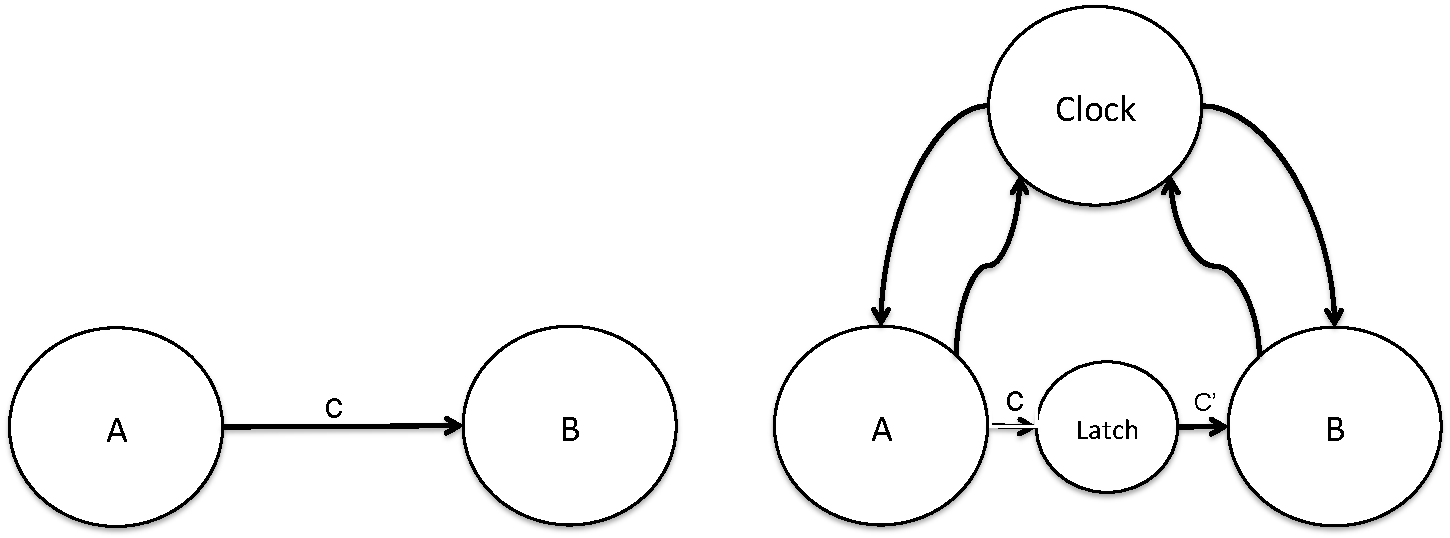
\includegraphics[width=10.0cm]{figures/clocked.pdf}
\caption{To enforce global synchrony on a simple reader-writer network in CSP, the complexity increase to include the clock and latch. Figure from \cite{Vinter2014}}
\label{fig:sme:clock_latch}
\end{figure}
\\\\
The advantage of using Python for this kind of processor simulation is the flexibility and simplicity of the language. It is easy to experiment with various ideas and versions but with the increased complexity of the added clock process and and clock-signal propagation, the advantages of Python seemed to diminish. Therefore the conclusion from the master thesis was that using PyCSP alone for building synchronous processor simulators was not feasible since the global clock was forced onto the CSP model. It was also concluded that external choice, which is a powerful and essential part of CSP, was not utilized in the globally synchronous approach. They did, however, conclude that several of other CSP concepts was fitting well with the hardware concepts, such as shared-nothing in CSP matches the structure of hardware communication.\\

After this attempt, it became clear that the structure of CSP was poorly suited for modeling clocked systems, and therefore it was decided to create the Synchronous Message Exchange framework, based on the CSP algebra. The idea was to only use the subset of the CSP algebra that provided beneficial functionality to hardware modeling which, most importantly, meant that external choice was omitted. However, the shared-nothing property of CSP showed to be very useful, since the network state could only be changed by process communication.
\\
% In SME the introduction of an implicit clock that eliminates the complexity caused by the model, described above, was imperative and is one of the key concepts hereof. The implicit clock removed the problems found by forcing the globally synchronous clock onto the CSP model. \\
In SME, a network is a combination of processes that are connected through buses. The processes communicate through a collection of signals in a bus, instead of CSP's synchronous rendezvous model, but retains the shared-nothing trait of CSP.
SME uses the term \texttt{bus} instead of \texttt{channel} to enforce the semantic correlation between the SME bus and a physical hardware signal bus.
The process communication is handled by a hidden clock which eliminates the complexity that arose from adding synchronicity to a CSP network. The combination of the hidden clock and the synchronous message passing between processes means that the SME model provides hardware-like signal propagation.

An SME clock cycle consists of three phases: it reads, executes, and writes as can be seen in Figure~\ref{fig:sme_process_flow}. The process is activated on the rising clock edge where it reads from the bus and it reads, executes and writes to the bus in one clock cycle. Just before the rising edge of the clock, all signals are propagated on all buses which means, that all communication happens simultaneously. Because of this structure, if a value is written by a process in cycle $i$, it is read by the receiving process in cycle $i+1$.

SME is able to detect read/write conflicts where multiple writes are performed to a single bus within the same clock cycle as well as reads from a signal that has not been written to in the previous clock-cycle.\\
All data, that are written to a bus can be logged for each clock cycle which means that these logs can be saved in a Comma-Separated Values, CSV, format and used for validating the VHDL implementation with a VHDL tool. This would eliminate the need to write seperate VHDL tests which will improve developer productivity immensely.

SME also supports clock-multipliers which means that a clocked network can have components inside the network being clocked at a different rate than its own clock. The rate can be an integer multiplier from its own clock. This means that all components are clocked relative to its parent network and therefore the clock will not need any extra coordination. It does however mean that the inner components can only fun faster than their parents.
% TODO: Do I really want this included?

Since an SME network is a network that can be represented as a graph, a diagram tool have also been implemented for SME. It utilizes the Graphviz tool to generate a visual graph of the network. This means that the SME networks can be generated and drawn as a graph which can help with debugging.
%TODO: Also, it this something I really want to include?


\begin{figure}[!ht]
  \centering
  \begin{tikzpicture}[auto]
    \node[mycircle, text width=2cm, shape=rectangle] (read) {Read};
    \node[mycircle, text width=2cm, shape=rectangle] (execute) [below=0.5cm of read] {Execute};
    \node[mycircle, text width=2cm, shape=rectangle] (write)  [below=0.5cm of execute] {Write};

    \draw [myarrow] (read) -- (execute);
    \draw [myarrow] (execute) -- (write);
    \draw [myarrow] (write) |-([shift={(5mm,-5mm)}]write.south east)-- ([shift={(5mm,5mm)}]read.north east)-| (read);
  \end{tikzpicture}
  \caption{SME process flow for one clock cycle.}
  \label{fig:sme_process_flow}
\end{figure}
Since SME is based on CSP, all SME models have a
corresponding CSP model, and because of this property, we are able to create a transpiler translating SME models to \cspm{}.
The SME model is currently implemented as libraries for the general-purpose languages C\#~\cite{Skovhede}, C++~\cite{asheim2015}, and Python~\cite{asheim2016vhdl}. The Python and C\# libraries both have code generators for VHDL as well.
\newpage
\subsection{SMEIL}
\label{SMEIL-section}
With the different SME implementations, a need arose for a common intermediate language. SME Implementation Language (SMEIL) was developed as a Domain Specific Language (DSL) for SME, usable both as an Intermediate Language, IL, and as an independent implementation language. It is accompanied with the implementation, \texttt{LIBSME}. %TODO: Find the reference in truls paper.
SMEIL has a C-like syntax with a specialized type system that makes hardware modeling simple. In spite of its simplicity, SMEIL still provides hardware-specific functionality that is more difficult to create with general-purpose languages.

Programs written in SMEIL are run by using the libsme library. This can be done either by using the command line utility or through the provided API.
The different methods of using SMEIL are:\\
\begin{itemize}
    \item \textbf{Pure SMEIL simulation:} A pure SMEIL program is a network which do not depend on outside influence. This means that the network  generates the data itself and the only communication are between the processes defined in the network.
    \item \textbf{Co-simulation of SMEIL:} The original intent with SMEIL was to create an intermediate language which could be used together with the general-purpose language implementations of SME, which is called co-simulation. With co-simulation, a test bench can be generated as well as VHDL code.
    \item \textbf{Direct code generation:} A SMEIL program which does not need to simulate before generating VHDL. In this case all types are constrained and all information needed for the code generation are in place. Because the simulation step is not executed, a VHDL test bench is also not automatically generated, since this happens in the simulation step.
\end{itemize}
The base entity of an SMEIL program is the module which corresponds to a file. The module consists of the actual SMEIL program as well as import statements. SMEIL programs can be seperated into modules which can then be importet into other SMEIL programs, creating a library-like structure and reusable components.\\

The SME model supports both synchronous and asynchronous processes. A synchronous process are run during every clock-cycle and an asynchronous process are only run when receiving a signal on the input bus, but unfortunately SMEIL does not currently support asynchronous processes. %TODO: Ask truls if it is implemented in other sme implementations.
\\

The two fundamental components of an SMEIL program is \texttt{process} and \texttt{network}. The process consists of variable and bus definitions, as well as the statements that are evaluated once for each clock cycle. The purpose of the \texttt{network} declaration is to define the relations between each entity in the program. A small example of process and network syntax can be seen in Listing~\ref{lst:smeil_small_syntax_example} and a further introduction to the language can be found in Section \ref{chap:analysis}.\\
\begin{listing}
\begin{minted}[escapeinside=||, mathescape=true]{smeil_lexer.py:SMEILLexer -x}
proc addone (in inbus)
    bus outbus {
        val: int;
    };
{
    outbus.val = inbus.val + 1;
}

    |$\vdots$|

network net() {
    instance a of addone(b.outbus);
    instance b of ..
    |$\vdots$|
}
\end{minted}
\caption{Small example of process and network syntax in SMEIL.}
\label{lst:smeil_small_syntax_example}
\end{listing}

\subsubsection{SMEIL type system}
The SMEIL language is stongly, statically typed and has a simple type system that is checked at compile-time. The purpose of SMEIL is to be able to model hardware, and since hardware is static, it was important to create a type system that was cabable of enforcing as many static invariants as possible. Therefore only between signed and unsigned integers is type coercion performed in SMEIL, which also means that only booleans can be used in conditionals.
It is easy to transform a statically typed language to a dynamically typed language, but not the other way around, therefore SMEIL will be simple to translate to various different target languages.

The SMEIL type system differs from standard general-purpose languages mainly on the support for bit-precise types. In general-purpose languages it is typical targeted a CPU which consists of fixed-width registers which typically means that it can not work with data smaller than a byte. This is, however, an important part of modeling hardware to be able to define the exact widths of the wires in order to optimise the hardware implementation. SMEIL supports unlimited-size integers as well as integers constained to a specific bit-length. SMEIL also supports booleans, double and single precision floating point numbers as well as strings. Currenly, floating-point numbers are not supported in the SMEIL hardware-translations. %TODO Venter på svar omkring hvad det her egentligt betyder? Og tjek lige at jeg ikke også skriver om det i analyse.
Arrays of a fixed length of the types, mentioned above, are also supported.

In SMEIL buses are represented as channel names and their types, and since processes or networks can accept buses passed as parameters it is important to ensure that no process or network is instantiated with a bus that does not contain the expected channels.
In the same way, it is essential to ensure that the directionality of the bus is enforced. When buses are passed as parameters, they are explicitly declared as either input or output bus. However, when defining a bus within a process it is not possible to define the directionality of the bus. Therefore the bus are defined as input or output based on their first use.
The type system of SMEIL is enforcing a set of rules that define how two buses are unified and the directionality of the bus, which ensures that problems such as the ones described above, does not happen.
All types of declarations in SMEIL are private exept bus declarations. As mentioned above, they are used for establishing communication between processes and therefore needs to be a part of the public interface of a process or network.

\subsubsection{Simulating SMEIL programs}
When translating SMEIL to hardware models, it is necessary to have all types in the program constrained to a specific width. However, as mentioned before, SMEIL does support unlimited size integers. Since it can be difficult to define an optimal width when writing the SME model, there was a need to provide both the support of the unlimited size integers while still being able to translate to hardware descriptions.
Therefore libsme provides a way to re-type the SME network based on the values that where observed during the simulation of the program.
During the simulation, the observed minimun and maximum value for all variables and channel are captured and saved along with the original value.
After the simulation, these minimum and maximum values are then converted into SMEIL types large enough to hold the range.
The new SMEIL program with the updated types and observed ranges are then passed through the type checker, in order to ensure that all constraints from the original program is still respected.
% An example of this can be seen in Figure \ref{fig:smeil_restricted_types_and_ranges} where a unlimited size integer is re-typed to an integer of fixed size after the simulation. In Figure \ref{fig:invalid} an example of a violation can be seen. Here the value c is contrained to \texttt{i10} but if the channel \texttt{b.chan} observe values that are 16-bit long then the restrictions on the c variable are violated.

% \begin{figure}
%   \centering
%   \begin{subfigure}[t]{0.25\linewidth}
%       \begin{listing}
%       \begin{minted}[escapeinside=||, mathescape=true]{smeil_lexer.py:SMEILLexer -x}
%           proc A ()
%            bus b {
%             chan: ?{\bfseries\underline{int}}?;
%            };
%            var c: i10;
%           {
%            c = b.chan;
%           }
%       \end{minted}
%       \end{listing}
%     \caption{Unconstrained types.}
%     \label{fig:oktype}
%   \end{subfigure}
%   \begin{subfigure}[t]{0.35\linewidth}
%   \begin{listing}
%   \begin{minted}[escapeinside=||, mathescape=true]{smeil_lexer.py:SMEILLexer -x}
%       proc A ()
%           bus b {
%               chan: ?{\bfseries\underline{i6 range 0 to 29}}?;
%           };
%           var c: i10;
%       {
%        c = b.chan;
%       }
%   \end{minted}
%   \end{listing}
%     \caption{Valid.}
%     \label{fig:non-violated}
%   \end{subfigure}
%   \begin{subfigure}[t]{0.35\linewidth}
%   \begin{listing}
%   \begin{minted}[escapeinside=||, mathescape=true]{smeil_lexer.py:SMEILLexer -x}
% proc A ()
% bus b {
% chan: ?{\bfseries\underline{i16 range 0 to 30717}}?;
% };
% var c: i10;
% {
% c = b.chan;
% }
%   \end{minted}
%   \end{listing}
%     \caption{Invalid.}
%     \label{fig:violated}
%   \end{subfigure}
%   \caption{Shows a process entering the simulator with an unconstrained type (a)
%     and examples of two possible resulting programs (b, c). The type changing
%     between the examples is underlined.}
%   \label{fig:simtyping}
% \end{figure}
% NOTE: THis figure does not compile. It is taken from Truls article and I should change the captions and also mention where I got it from.

% In Figure \ref{fig:smeil_restricted_types_and_ranges} the two last programs, showed in Figure x and y, will be the result of the re-typing of the program after simulation. That is, the programs resulting from the simulation of the program in Figure z.


\subsubsection{Co-simulation}
Often when modeling hardware in Hardware Description Languages (HDLs) like VHDL or Verilog, code for testing and verifying are often written in the same language as the design itself. Unfortunately, the HDLs often does not have the functionality for generating proper simulation input. Using general-purpose languages for testing hardware models are useful since the range of available libraries are much larger.
Therefore the SMEIL simulator provides a simple language-independent API which enables SME implementations written for general-purpose languages to communicate with SME networks written in SMEIL, so-called co-simulation.
The big advantage of the SMEIL approach to co-simulation is that SME is used on both sides of the co-simulation and therefore both sides acts as a single entity.
The PySME %TODO: Reference
library have been extended to support co-simulation with SMEIL, thereby providing the posibility of writing networks in PySME which can interact with SME networks written in SMEIL. Currently, this extension have only been implemented in the PySME implementation, but is expected to be implemented in the other SME implementations as well.\\
Another functionality of the libsme compiler is, when simulating the SMEIL network, the compiler can record a trace of all communication between processes in the network. This trace file can then be used as a source for the VHDL test bench which can be used to verify the generated VHDL code.

% Some parts of the SMEIL grammar is not implemented in SMEIL yet and therefore we are also not supporting these.
In Figure~\ref{fig:smeil_transpiler} the SMEIL transpiler structure can be seen.

\begin{figure}[!ht]
  \centering
  \begin{tikzpicture}[auto]
    \node[mycircle, minimum size=1.75cm, align=center, text width=1.75cm, font=\footnotesize]    (smeil)                                       {SMEIL};
    \node[myrectangle, text width=1.5cm, minimum height=1.0cm, inner sep=5pt, inner ysep=5pt] (csme)  [above left=-0.25cm and 1.5cm of smeil] {C\#SME};
    \node[myrectangle, text width=1.5cm, minimum height=1.0cm, inner sep=5pt, inner ysep=5pt] (pysme) [below left=-0.25cm and 1.5cm of smeil] {PySME};
    \node[myrectangle, text width=1.5cm, minimum height=1.0cm, inner sep=5pt, inner ysep=5pt] (vhdl)  [right=1.0cm of smeil]                {VHDL};

    \draw[myarrow] (csme)  -- (smeil);
    \draw[myarrow] (pysme) -- (smeil);
    \draw[myarrow] (smeil) -- (vhdl);
  \end{tikzpicture}
  \caption{SMEIL transpiler structure.}
  \label{fig:smeil_transpiler}
\end{figure}




\newpage
\section{CSP}
Communicating Sequential Processes (CSP) \todo{reference} is a process algebra that provides a way to express interaction between processes of concurrent systems.
CSP had a lot of influence in the design of the programming language Occam as well as the Go programming languages and several other. As described in Chapter \ref{chap:related-work}, it was first itroduced in 1976 by C.A.R Hoare but only later on did it develop into a process algebra. CSP is still the subject of research and due to the tools available today, it is increasingly becomming a more accessable tool for the interested user.

CSP provides the posibility of describing systems in terms of message passing communication between independently operating processes. The \textit{sequential} part of the CSP name is not exactly applicable anymore, since the current version of CSP allows not only sequential processes, but also processes consisting of parallel compositions of other primitive processes.
By using message passing between processes the language avoids certain problems that arise with the use of e.g shared variables.
With the use of the process algebra of CSP, it is possible to describe complex parallel structures with a few simple elements of the algebra.

The two fundamental parts of CSP are \textit{Events} and \textit{Primitive processes}. \textit{Events} are the communication between processes. They are instantanious and can be simple names, like \textit{clock} or compositioned names, like \textit{add.kill} or it could be input/output events, like \textit{add ? x} or \textit{hours ! y}. %TODO: This section is a bit too much like the wikipedia version, this should be rewritten
The \textit{pimitive processes} are consisting of processes which have basic behaviour such as \textit{STOP} or \textit{SKIP}. The \textit{STOP} process is a process that simply does nothing, not even terminate, and it is also called deadlock. The \textit{SKIP} process is the process that terminates successfully.


% ------
%TODO: Figure out if this should be here or somewhere else in the report
CSPs different algebraic operators are used to define the different relationships between processes in CSP.
\begin{itemize}
    \item \textbf{Prefix:} The prefix operator link an event and a process.
    $a \rightarrow P$ defines a process which will communicate $a$ and then behaves like the proces $P$. The process will wait indefinitely until communicating $a$.
    \item \textbf{Deterministic choice:} Also called external choice is the operator which offers the environment the choice between two different processes. $(a \rightarrow P) \square (b \rightarrow Q)$ in this example the environment choose to either perform event $a$ and then behave as the process $P$ or perform event $b$ and then behave as the process $Q$.
    \item \textbf{Nondeterministic choice:} Also called internal choice, defines the choice between two processes but is not affected by the envionment to make the decision.
    $(a \rightarrow P) \sqcap (b \rightarrow Q)$ can perform event $a$ or $b$ and then behave as the corresponding process, but it does not have to accept either. It is only required to accept one if the environment offers both of them.
    \item \textbf{Interleaving:} This operator represents concurrent activity between two independent processes. $ P  |||  Q$ defines a process behaving like $P$ and $Q$ simultaneously.
     \item \textbf{Generalised parallel:} This operator represents two processes concurrent activity but where the processes are required to syncronise on the set of events, defined in the operator. $ P  |[\{ a \}]|  Q$ defines the process where $P$ and $Q$ must syncronise on event $a$ before the event can occur. All events not defined within the synchronisation can happen at any given time.
     \item \textbf{Hide:} This operator represents a process which performs any event from the set defined, but the event is hidden and becomming an internal event, a \textit{tau}.
\end{itemize}

% -----
% TODO: Written a lot like the wikipedia page. This require a rewrite!
There are three denotanional semantics models in CSP, which are the \textit{traces} model, the \textit{failures} model, and the \textit{failures divergences} model. The \textit{trace} model define a process expression as a set of sequential events, traces, that the process can perform. $traces(STOP) = {<>}$ means that the trace of the process \textit{STOP} is the empty set, since the process performs no events. $traces(a \rightarrow b \rightarrow STOP = \{<>, <a>, <a,b>\})$ means that the trace of the process defined above can either be no events performed, the event $a$ performed or both event $a$ and then event $b$.\\
The failures model is similar to the trace model, but consists of a set of refusals, which are the set of events that a process can refuse to perform. A failure consists of both a trace and a set of refusals, which identifies the events that the process can refuse when it has executed the trace. $failures((a \rightarrow STOP) \square (b \rightarrow Q) = \{(<>, \emptyset), (<a>, \{a,b\}), (<b>, \{a.b\})\})$\\
The last model, the \textit{failures divergences} is en extension of the failures model. The model is defined as a pair... %TODO: Explain better, the wikipedia site is weird and I dont really understand it. I should understand what I write!

\subsection{\cspm{}}
%CSPm was devised by Bryan Scattergood as a machine-readable dialect of CSP  - se the paper \textit{The Semantics and Implementation of Machine-Readable CSP}\\\\
\cspm{} is a formal language that combines CSP with a functional programming language in order to make it easier for the programmer to model the systems and then use the code on tools that can animate, verify or similar.


\subsection{FDR4}
%" FDR2 is often described as a model checker, but is technically a refinement checker, in that it converts two CSP process expressions into Labelled Transition Systems (LTSs), and then determines whether one of the processes is a refinement of the other within some specified semantic model (traces, failures, or failures/divergence)" (from Wikipedia - se paper \textit{Model-checking CSP - af Roscoe} \\\\
FDR (Failures Divergence Refinement) tool is a refinement checker for

In the paper \textit{A primer on model checking}\cite{Ben-ari2010} Mordechai Ben-Ari explains a concurrent problem that he had used for many years, to teach his students about concurrency. ... % TODO: write this when I have read the article again


We not only want to transpile SMEIL to \cspm{}, we also want to be able to verify different properties in \cspm{} in order to prove correctness. Today, there exists several tools for formal verification, both in academia and in the industry. One of the currently most favored tools is the Failures-Divergences Refinement tool (FDR4). This tool is a CSP refinement checker that can analyze programs written in the machine-readable version of CSP; \cspm{}.
It provides a parallel refinement-checking engine that can scale up linearly with the number of cores. This means that it can handle processes with a large number of states in a reasonable time. FDR4 can handle several different types of assertions, deadlocks being the most used. However, due to the structure of SMEIL, we use FDR4 in a different way than is typical. Since the SME model cannot have cyclic-wait we have no need to verify the system in this manner.

For our current implementation of the transpiler, we can assert the ranges of the channel inputs, for example, we can automatically assert that the observed ranges, provided by the SMEIL simulation, and the possible input on the \cspm{} channels are not conflicting.
In hardware, we would typically want to verify that the communication on a bus does not exceed a certain range or that the sum of multiple signals does not exceed a specific value. A bus might be able to carry other data than needed, and being able to model a circuit that can assert that the bus never carries other data than expected, is of great value.
\\

CSP was not initially developed for hardware modeling, and therefore it is not evident how to handle the clock cycle, which is an essential part of hardware modeling. When we transpile the SME network into \cspm{} the SMEIL simulation have provided the ranges of all values from the simulation and therefore all clock cycles. This means that when FDR4 asserts a property it asserts on all possible communication combinations for all the simulated clock cycles. Therefore, even though we are transpiling from an SME model, where the clock is crucial, we can simply translate ``one-to-one" from the SMEIL program and still get an accurate assertion on the properties.

